\section{Inheritance}
\subsection{Variation}

Variations are the differences between individuals of the same species. They can be of two types:
continuous and discontinuous. 

Continuous variation is that where there is a range of different phenotypes (expressions of genes)
and discontinuous is that where there are distinct categories of phenotypes. Examples of the two
are height and ABO blood groups, seed shape and colour in peas, respectively. Discontinuous 
variation tends to be the result of genes and genes only, whereas continuous variation results from
both genes and affects of the environment.

\subsection{DNA}

The structure of DNA consists of two coiled strands, forming a double helix, where each strand is
made up of a chain of nucleotides\footnote{The monomer unit of DNA.}. Each nucleotide has a base,
one of: A, T, C or G. Bonds between the bases on either strand hold the strands together in the
helix structure. The bases always bond in the same way; A with T and G with C.

A gene is a length of DNA that codes for a specific protein. As a result, DNA controls a cell's
function by controlling protein production, including proteins such as enzymes. 

The sequence of bases in DNA determines the sequence of amino acids needed to make a specific
protein. The sequences of the amino acids in a protein is what gives proteins different shapes.

\subsection{Inheritance}

Inheritance is the transmission of genetic information from generation to generation. An allele is
an alternative form of a gene.

The genotype of an organism is the genetic makeup of the organism in terms of the alleles present,
for example lets have two alleles, dominant and recessive, be G and g. The genotype of an organism
may be Gg. The phenotype of an organism are the observable features of the organism, which are
results of the genotypes. A dominant allele is that which is expressed in its presence, always
denoted by an uppercase letter, and a
recessive one is that which is only expressed when there is no dominant allele of the gene present
and is always denoted by a lowercase letter.

A homozygous combination of alleles is that where both alleles are the same (GG) and a heterozygous
combination of alleles is that where the alleles are different (Gg).

We can predict the genotypes of offspring from the phenotypes of parents. An example follows:

\begin{center}
\begin{minipage}{0.8\textwidth}
The gene for black hair in humans is B, and is dominant over that for red hair, b. What are
the chances of the phenotypes for the offspring of two parents who are red haired and 
black haired, the latter having a heterozygous combination?

Note that, the red haired parent's genotype must be gg and the black haired parent's must be Gg.
Using this information we can compose a Punett square:

\begin{center}
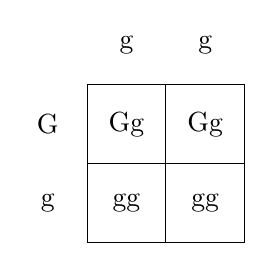
\begin{tikzpicture}
    % Draw grid
    \draw (0,0) grid (2,2);
    
    % Labels for parents
    \node at (-0.5,1.5) {G};
    \node at (-0.5,0.5) {g};
    
    \node at (0.5,2.5) {g};
    \node at (1.5,2.5) {g};
    
    % Offspring combinations
    \node at (0.5,1.5) {Gg};
    \node at (1.5,1.5) {Gg};
    
    \node at (0.5,0.5) {gg};
    \node at (1.5,0.5) {gg};
\end{tikzpicture}
\end{center}

Where, we see 2/4 outcomes are Gg and 2/4 outcomes are gg. We can deduce that there is a 50\% 
chance of the offspring being black haired in heterozygous combination and that there is a 50\%
chance of offspring being red haired in homozygous combination We can deduce that there is a 50\% 
chance of offspring being red haired in homozygous combination.
\end{minipage}
\end{center}
The results of a genetic prediction such as the above are only probabilities, which are never
perfectly accurate, especially for small numbers of offspring.

Two identical homozygous individiuals will be pure-breeding, in that any and all offspring will
inherit the exact same genes as shown below:
\begin{center}
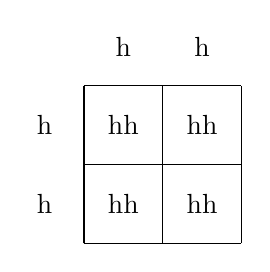
\begin{tikzpicture}
    % Draw grid
    \draw (0,0) grid (2,2);
    
    % Labels for parents
    \node at (-0.5,1.5) {h};
    \node at (-0.5,0.5) {h};
    
    \node at (0.5,2.5) {h};
    \node at (1.5,2.5) {h};
    
    % Offspring combinations
    \node at (0.5,1.5) {hh};
    \node at (1.5,1.5) {hh};
    
    \node at (0.5,0.5) {hh};
    \node at (1.5,0.5) {hh};
\end{tikzpicture}
\end{center}
Notice all resulting offsprings have the same allele combination as both parents.

Codominance is that where alleles that are both expressed in the phenotype when they are both
present in the genotype. This is seen in the ABO blood group system in humans, where the alleles
for the A blood group is codominant to that for the B blood group.

There are three alleles for blood groups: A, B and O, shown as I$^{\textrm{A}}$, I$^{\textrm{B}}$
and I$^{\textrm{O}}$. The I$^{\textrm{O}}$ allele is recessive to both the I$^{\textrm{A}}$ and
I$^{\textrm{B}}$ alleles.

\begin{center}
	I$^\textrm{O}$I$^\textrm{O}$ gives phenotype of blood group O.

	I$^\textrm{A}$I$^\textrm{O}$ gives phenotype of blood group A.

	I$^\textrm{B}$I$^\textrm{O}$ gives phenotype of blood group B.

	I$^\textrm{A}$I$^\textrm{B}$ gives phenotype of blood group AB.
\end{center}

In humans, gender (sex) is determined by the last pair of chromosomes, the twenty third. Males have
chromosomes shaped like an X and a Y, and they are named accordingly, the XY chromosomes. Females
have sex chromosomes shaped like two Xs, which are hence named accordingly, XX. Using a Punnett
square, we see that the chance for the child being either of the two sexes is 50--50.

Gene mutation is a random change in the base sequence of DNA. This may result in certain diseases
such as sickle cell anaemia, where, due to a change in the gene responsible for producing red blood
cells, the red blood cells are shaped like sickles and this affects individuals' ability to absorb
oxygen.

A chromosome mutation is that where the number of chromosomes is affected. An example is Down's
syndrome, where an extra chromosome in the twenty-first pair of chromosomes causes the individual
to be intellectually and physically challenged. In such a condition the total number of chromosomes
is 47.

Mutation is the reason behind genetic variation in populations. The random change in DNA sequence
results in a different amino acid being synthesised from that gene. Hence a different phenotype
arises. As seen before, gametes are haploid cells which are produced by meiosis, which means half
of the alleles of the parent individual is contained in the gamete. Which half exactly, is
random, and when two gametes fuse, the combination of alleles can be unique, producing variation.
Furthermore, which individual's allele combines with which depends on which parent mates with which,
a matter which produces new combinations of alleles.

Lastly, ionising radiation and some chemicals increase the rate of mutation.

\subsection{Selection}

In a population, there will be variation in phenotypes. Many offspring will be produced, with those
variation, and they will struggle amongst each other to survive, competing for food and resources.
Those who are adapted to the environment will survive, and will go on to reproduce, passing on 
their genes to their offspring which will hence also be well adapted.

As a result, the inherited features of a population can evolve over time, depending on changes in
environment. It may also occur that, a genetic mutation results in a phenotype which is more well
adapted to a certain environment.

Humans can selectively breed species. We can select animals or plants with features we desire, and
make those breed (cross them) to produce the next generation. We will select the offspring showing
those desirable features and this will repeated over many generations.

Artificial selection is important to produce plants and animals that are economically important. For
example, disease resistant foodstock can be produced in this way.
